\documentclass[14pt]{extarticle}
\usepackage[utf8]{inputenc}
\usepackage{amsmath}
\usepackage{graphicx}
\usepackage{hyperref}
\usepackage{float}
\usepackage{listings}
\usepackage{color}
\usepackage{minted}


\title{MASCWave}
\author{Muhammad Z Ilahee }
\date{Feb 2018}

\begin{document}

\maketitle
\section{Abstract}
MASCWave is an online tool for rendering digital timing diagrams and other technical visualization which are formatted as HTML SVG elements and can later be downloaded as an SVG or PNG image. The platform is based on on the free open source WaveDrom project and modified to manage bigger timing diagram data integrated with Socketio module in nodejs. This paper provides an analyzation of how the timing diagram data is formatted, parsed, rendered and accommodated for suitable view. This paper also provides a short tutorial on how to utilize this tool. 
\newpage

\section{Introduction}
 Digital timing diagram represents an arrangement of signals in it’s time domain. A typical timing diagram contains signals mostly consisted of digital waveforms in multiple rows marked by the vertical time lines. A digital timing diagram is often useful for debugging simulations, designing chips, diagnose digital logic hazards etc. There have been number of tools around to analyze a digital timing and many of them are open source and free to use. This paper describes such a tool called MASCWave created for online viewing of digital waveforms. MASCWave is a server based web app which is built over WaveDrom library and provides multiple functionality in addition to existing WaveDrom features. The main focus for MASCWave is to provide an online tool for analyzing Waveforms from any platform that supports the standard modern browsers. It’s frontend is designed with HTML5 and it’s backend is npm and JavaScript based. It can render digital timing diagrams for any properly formatted WaveJSON files and is flexible on updating the rendered diagram without the need of modifying the HTML. A specially formatted WaveJSON file is uploaded which is parsed by the server, turned into a  JSON variable and a portion of that JSON variable is sent to the client for visualization. Then that portion of the variable is rendered by the WaveDrom library for visualization.

 After the JSON variable is rendered the user can highlight multiple waveforms by selecting them. They can also view every single wave individually and get information about them. There is functionality to navigate the time to view waves prior to or after the current time. If there are multiple wavelanes which can not viewed in the current window space, then the user is able to navigate up and down to view more of the waves. As an added feature we have a text box where we could input a javascript function that returns an array of data and we can show that in the visualization pane. If the user is interested to save the current view, there is a functionality to save the image as png and download it.
 
 This web app is also based on real time user interaction independent of HTTP GET or POST requests. It initiates a socket connection with the server using SocketIO for communication.  So when the user requests more data from the waveform or more wavelanes it doesn’t submit an HTTP request thus the user session isn’t terminated. Moreover, it has caching mechanism so if at any point the user loses connection to the server while working on a waveform, the user can pick up their last waveform based on their browser cache.

\section{Acknowledgement}
This project is supervised by Professor Jose Renau and his MASC group at UCSC. Nursultan Kabylkas, one of the members of the MASC group, provided the necessary wave dump files for testing and debugging the web app. Professor Guthaus provided support on the thesis. Finally, a special thanks to the WaveDrom project ( \url{http://wavedrom.com/} ) and SocketIO (\url{https://socket.io/} ) since the core of the project was built using these libraries.

\section{Related Works}
\par GTKWave, WaveDrom, LaTeX typesettings,Epwave are some of the most useful ones that are used as waveform viewers. Each of them has their own pros and cons.
\par WaveDrom is designed to work with web browsers and thus it is available online without requiring the user to download a software or app on their devices. It takes a WaveJSON formatted string which is parsed as a JSON variable and rendered in the web browser to show the waveforms. Moreover, it has cross platform stability and it is compliant with major web browsers. The users can also download the waveform after it's generated. However, there is an issue with the barebone WaveDrom structure. WaveDrom is not supported by a backend and it tends to break for larger signal data. It also doesn’t have select ability of individual waves, capability to easily identifying a wave, changeability of an existing diagram, uploading capacity of a pre-formatted data file and scrolling capability through the timing diagram based on a given time frame. Moreover, WaveDrom isn’t supported to render waveforms given an uploaded source code. 

\par GTKWave is a fully featured GTK+ based wave viewer for Unix, Win32, and Mac OSX which reads different fortmats of files as well as standard Verilog VCD/EVCD files and allows their viewing. It also allows the users to navigate and zoom. There's also functionality for saving the generated waveforms for using in documentation. GTKWave provides support for some of the shortcomings of WaveDrom but it’s not available online and requires the user to download and install the software. GTKWave also doesn't allow tight code visualization where users can upload source code and thus the waveform would be generated. GTKWave source code is available but it would be difficult for user to make it available on their web browser.  The users are also not capable to highlight a single or group of waves which might be particularly interesting to them and there is no way users are able to visualize the properties of any of the waves.
\par LaTeX typesetting is used in LaTeX documentation for publication quality waveforms based on textual markup as source for the waveform. While this is good for documentation purposes, it has a shortcoming. LaTeX waveform shows only certain timeframe for using as a figure in a document and it is not meant to be interactive. Moreover, one needs to know LaTeX very well to code and generate the waveforms. Since this is not interactive, many of the options to expand the view of a given wavedump file is also missing here.
\par Epwave is probably the closest to what WaveDrom can do and it's also easy to use. It is available online and it can take either a link with a wavedump or an uploaded file with wavedump in vcd format. It let's user navigate the waves left and right, zoom in and out on the waveforms and add or remove waveforms. It is also capable of saving the user progress and lets the user pick up from where they left off. However, there are couple setbacks to this amazing tool. First of all, the source code isn't publicly available thus there is no place for customization or modification instead of using the EDA playground website. So if any industry wants to visualize their waveforms in an intranet setting, they would have to upload their waveform file to the EDA website. It also doesn't have code evaluation capability so if someone is willing to compile their own source code for tight visualization, they are unable to do so. Also if someone would like to make modification to the backend to suit their requirements they are unable to do so. Individual waveforms are also not selectable and the properties of each of such waves are not viewable by the user either. Also other than taking screenshots, there is no way users can save or download the waveform.

\par Thus we considered all of these deficiencies and created MASCWave which addresses all of these issues along with the existing features available. MASCWave is designed with a client server based model where the communication is done over socket rather than any HTTP GET or POST request. This behavior allows the user to send navigate, zoom, select or such commands without refreshing the page as the communication doesn't require the processing of extra protocols other than TCP. The sockets are well secured and only one client is capable of having one socket per session and no two clients can share the same socket. The dump files are uploaded to the server over express server which is powered by nodejs. The data is transferred over web socket. The user session is also tracked by the server using web cache thus the user doesn't have to upload the Wavedump file multiple times to generate the waveform. Once the waveform is loaded users can navigate the waveform left and right and only the selected amount of data is transferred from the server instead of the entire waveform. Users can zoom in and out and they can also hover over waveforms to see the properties of each individual waveform. If any particular waveform or group of waveforms interest the users they can also select and highlight those waveforms and those  highlights will stay for the entire session. There is also option for users to download the generated waveforms. The biggest difference between all the existing tools and MASCWave is the tight visualization tool which allows users to upload their own code which returns an array and let's them visualize it. 

\section{Work Flow}
\par There are 3 main flow of the entire tool. Server side processing, Client side interaction and Client side rendering. Each of the phases are described here with their respective work flow diagram. All methods of communication between the client, client rendering and server is done over a massive json object called client data containing data about different properties of the waveform, session id, client information, client code submission data etc. The data is stored in a waveJSON formatted file known as a wavedump file.

\subsection{Client Side Flow}
\begin{figure}[H]
    \centering
    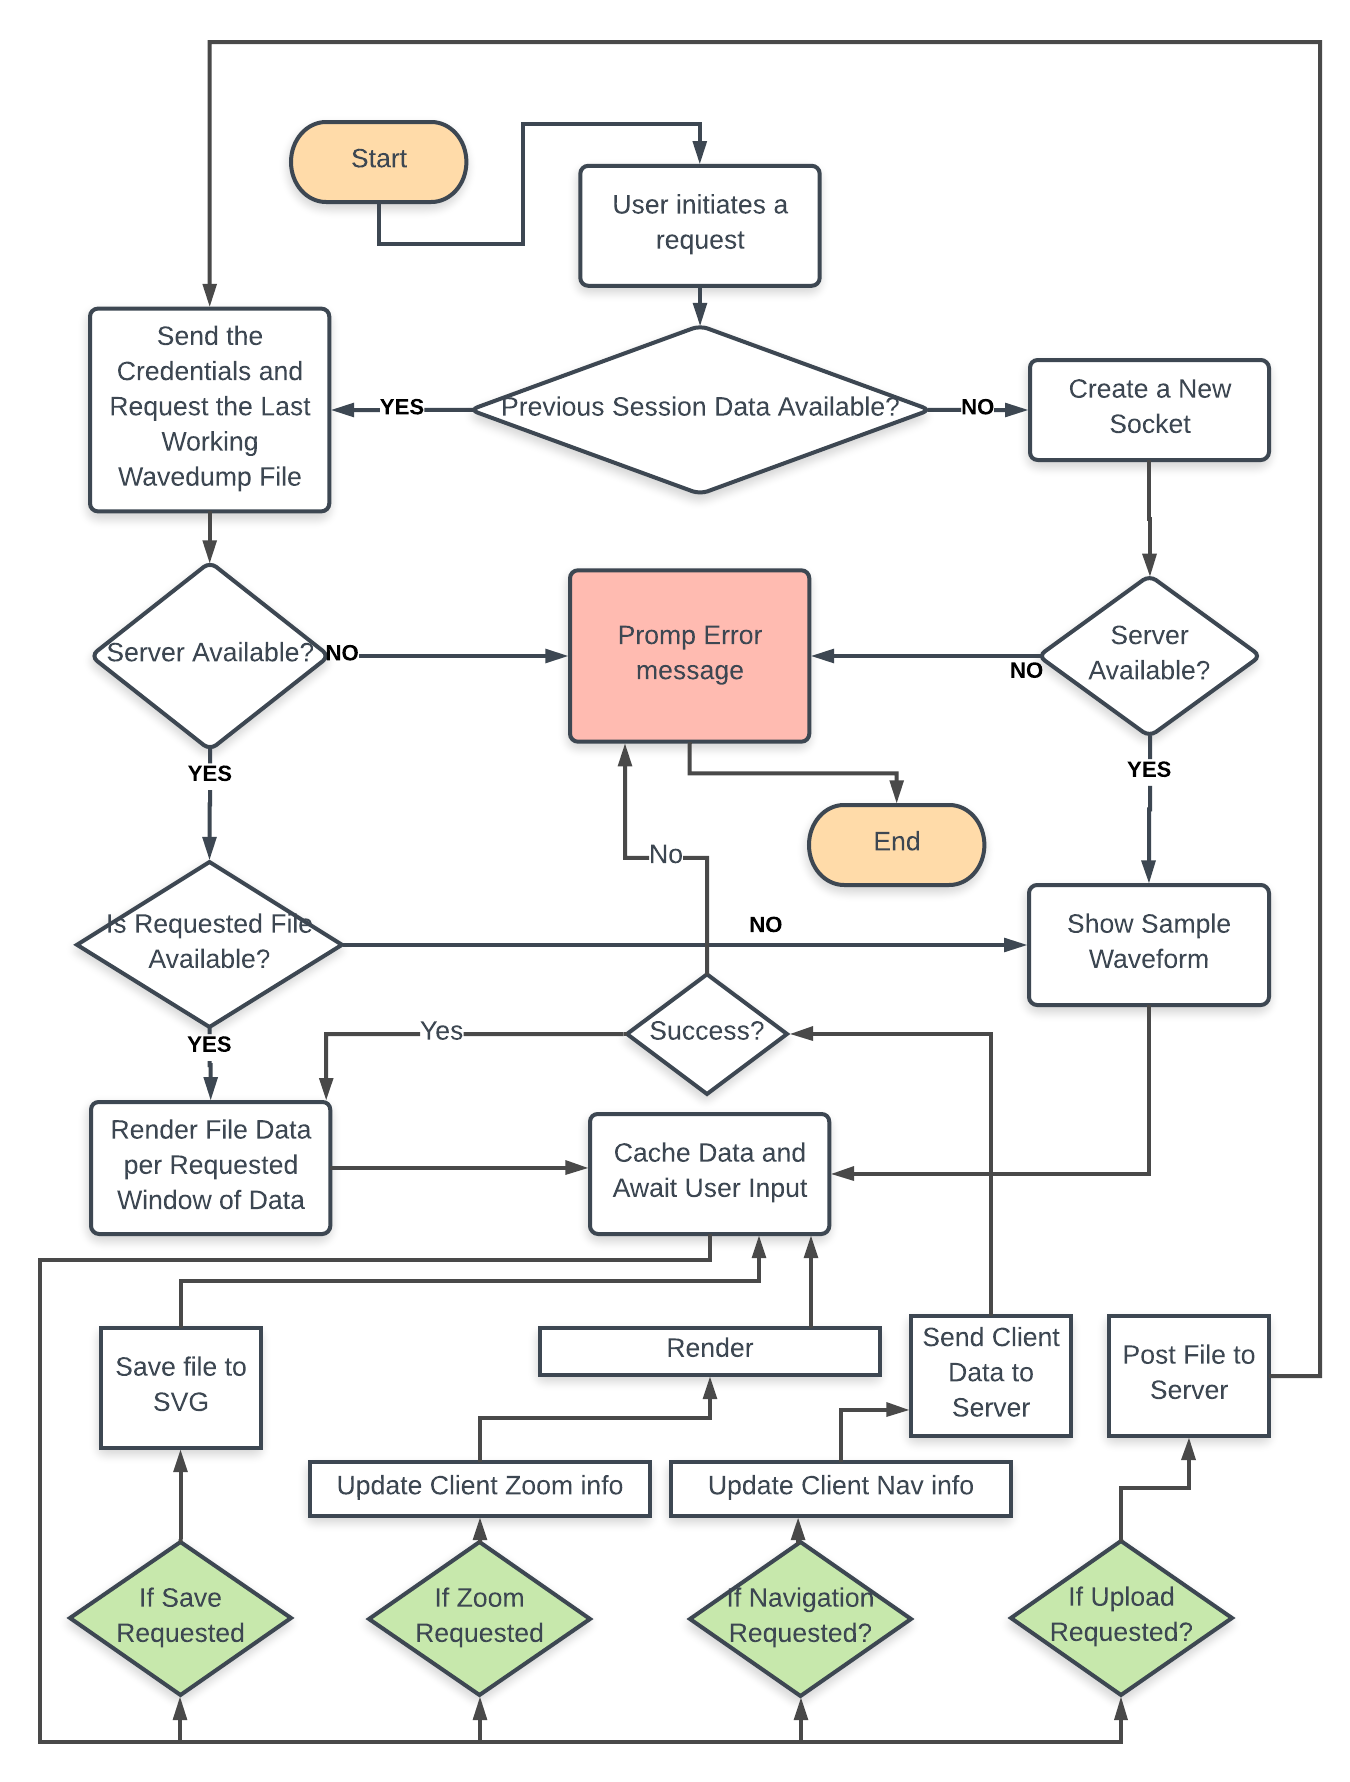
\includegraphics[scale=0.25]{client}
    \caption{Client Flow Chart}
    \label{fig:Client Flow Chart}
\end{figure}
\newpage
\par When a user tries to access the website, a new request is initiated from the client side (web browser) and the client side queries whether the previous session info and data are cached or not. If previous data is not available then it creates a new socket connection with the server and checks whether the server is available. If the server is inaccessible during that time, then the page will prompt an error message to the user showing that there was an issue creating a new connection.
\par If the server is available then the client requests the necessary files needed for rendering. The details about the the file transfer would be mentioned in the section Server Side Flow. The initial HTML file contains a placeholder waveform available for the user to see as an example and it provides user the options to upload file, upload JavaScript code, save the current waveform, navigate left or right to see more waveforms and navigate up and down to see more wave lanes. The client data is cached which includes the session id, id of the client, and some more details about the waves including the position of the waveform being viewed, selected waveforms' id, zoom info on the waveform etc. The client awaits the user to select any of these inputs while keeping the connection alive. 
\par In the case where there was previous session data available to use, the client would pull those from the cache and check the server connection. If the server doesn't respond back then an error would be prompted. If the server responds back, the client connects to the server over web socket and send the existing data requesting the file where it left off. Although it would create a new web socket with a new id, the client would send the existing session id to the server to identify itself as an older user and if the information is available in the server then the server will hand off the previous data. The data is set to be stored securely for 3 days as well as the cached client data until it's expired and removed from both the client and the server. Details about how the data is stored in the server is mentioned in the section Server Side Flow.
\par After identifying itself to the server, the client requests the wavedump file it was working on previously. During this process the client also sends information about how much of the data is needed by the client by sending the window size information. If the client is zoomed out then it will ask for more data while if the client is zoomed in, it would require less data. Once the server sends the necessary amount of data, it goes through the rendering process and if there is no error in the data, it is rendered on the wave window. To see how the rendering is done, check the section Client Side Rendering. To see how the data is sent from the server to the client check the section Server Side Flow.
After the rendering is done, the client updates the client data and caches it. It then waits for the user to give some input.
\par There are 4 different types of interrupt done by the user, request to save the waveform to an svg file, request to zoom in or out, request to navigate horizontally or vertically, request to upload file or code. Some of them require interaction with the server while the others are just done locally through render.
\par When a user request to save the file, the rendering process finds the part of the webpage that holds all the waveform and converts them into a file. Details about the entire process is mentioned in the Client Side Rendering. Then the file is linked to the save button for download and thus the user can get the current window as an SVG file. When a user requests to zoom into the waveform the rendering process chooses the appropriate waveskin file depending on the the amount of zoom and refresh the page without the need of resetting the connection or communicating with the server. The client simply sets the window size to be smaller or larger inversely. For example, if the user requests to zoom in, since the display size would be the same the client would decrease the window size to fit the object in that display.

\par When the user chooses to navigate left or right this also doesn't require server communication as the server sends the entire wavelane data at time but to cut down the amount of data sent by the server, trimming the amount of horizontal data would be introduced. See the section Future Work for more details. When the horizontal navigation request is made, the rendering process validates the window size and renders only the data requested by the client through the user request. This way it doesn't take longer to render the entire wavelane and thus cuts down the processing time. The amount of navigation could be changed based on the user input.

\par When the user chooses to navigate up or down to view more of the wavelanes in the wavedump file, the client sets the vertical start variable in the client data to the desired value and send the information to the server. The server then validates the request and sends back the chunk of data requested by the user. The data is then rendered accordingly. Alike horizontal navigation, vertical navigation size could also be selected by the user.

\par When the user has a wavedump file that they want to view, it is uploaded to the server from the client. When the user selects and uploads the file to the server, it is validated and stored in the server and only the initial chunk of data is sent to the client. When the user wants to upload code for tight visualization, the client takes the code and stores it in the cache first before sending it to the server. The reason behind caching is since uploading any data to the server is done through HTTP GET or POST request, the connection reset by the server when it redirects the client to the home page and any data which is not cached will be lost. So to pertain the code written on the code pane, it is a good idea to store it locally.

\newpage
\subsection{Server Side Flow}
\begin{figure}[H]
    \centering
    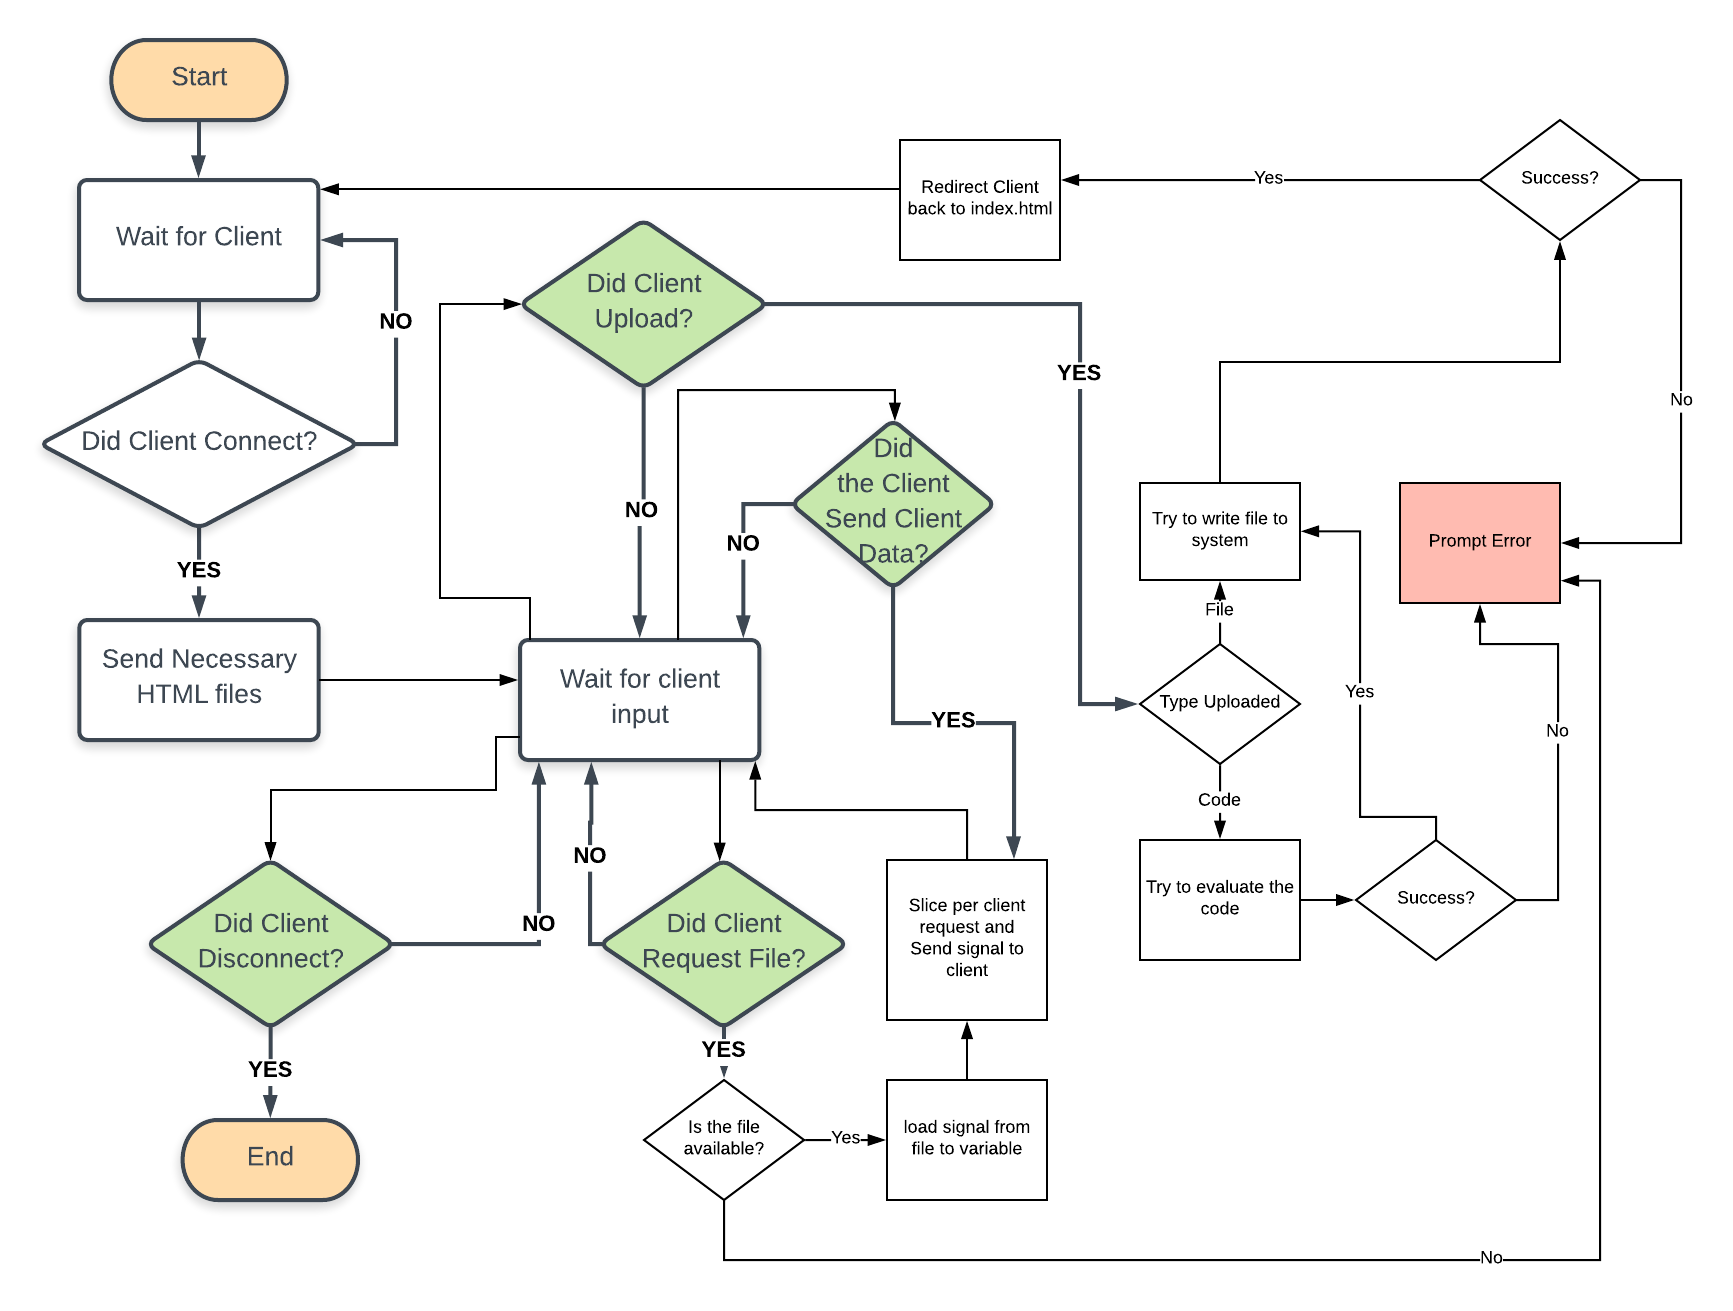
\includegraphics[scale=0.23]{server}
    \caption{Server Flow Chart}
    \label{fig:Server Flow Chart}
\end{figure}
\par The Server is started by invoking npm packages which create a file server and a web socket together. The file server is powered by express.js and it provides to functionalities - ability for the user to upload files and sending necessary files for the webpage once a client connects. The express file server is the bridge between users and server for file storage. While serving files per user need, it also validates whether the file upload was successful or not.
\par The server awaits to get a connection request from a client and listens to the designated port. When a client connects to the server,  necessary html files, css files and javascript files are provided. For developers, if they want to serve more files they would need to modify it by adding the filenames to the sendFile function. Once all the files are transfered to the user, the client processes them and renders them for the user to view and loads the inputs to interact with the server. It then creates a web socket for the client. Then the server waits for the client inputs. 

\par There are 4 possible cases while the server awaits client input. They are client file request, client disconnection, client upload, and  client data handle. 

\par If the client had connected to the server in the past the server creates a file for that client ID which is stored in the server for 3 days before it is removed. If the file has been accessed any time before the 3 day period ends, the lease is renewed. The client will retrieve the old ID from it's cache and send it to the server. More details about that is mentioned in the section Client Side Flow. The client then sends the data packaged in a json variable over the newly created web socket. One issue with web sockets are they are not cachable or retrievable once the connection is dropped. For example, if Client A is connected to server with a session id s55FlaWwr7Eju4qeAAAE and later the client disconnects from the server, socket io will not keep the connection alive for the client and the id will be gone. The client would not be able to get the same id again. This is because of security and to prevent spoofs and man in the middle attack. That's why to retrieve the information client would need to cache the working session id for future reference. 
\par Once the client data is sent to the server, the server tries to retrieve the id from the data and tries to validate it to the files stored in the memory. If a file associated to the id is not found then the server would not consider that as a returning client and would wait till the client uploads a source or file. If the id matches a file then the server would recognize the client and validate rest of the client data. In this step the server would check the clients data for the data chunk requested. Then it would parse the data file, slice the chunk of data needed by the client and send it to the client. 

\par Every time in the future when the client sends client data, the server would validate the data in such a way and send the requested chunk to the client. If at any point the client sends an invalid data or an out of the bound data request, the server would ignore the request and catch the error. If the server debug mode flag is active, then it would also print the error to console.

\par When the client uploads something, the server checks whether it is a code or a WaveJSON file. If no file is found with the request then the server would check for code. The code is split up into wave lanes and evaluated. If an error occurs the server would catch that and wouldn't return any data to the client. The server would consider everything as an error except for the fact that the code returns an array of data. If the evaluation is done properly then the server would convert the output into a waveJSON format and store it to a file. The filename would be determined from the client id that is retrieved fromt the client data object.

\par When the server finds a WaveJSON file, it would then validate whether the file is a text file or not. If a text file is not received then the server would ignore the file and redirect the client back to homepage and would not store the file. If the file is a valid text file then it would be stored in the tmp directory under the server directory in the server and will be stored there for 3 days. The file would then go through the same process as client data handling and if there is no error, chunk of the data from the file would be sent to the client for visualization where client side rendering would process the data.


\subsection{Client Side Rendering}
\begin{figure}[H]
    \centering
    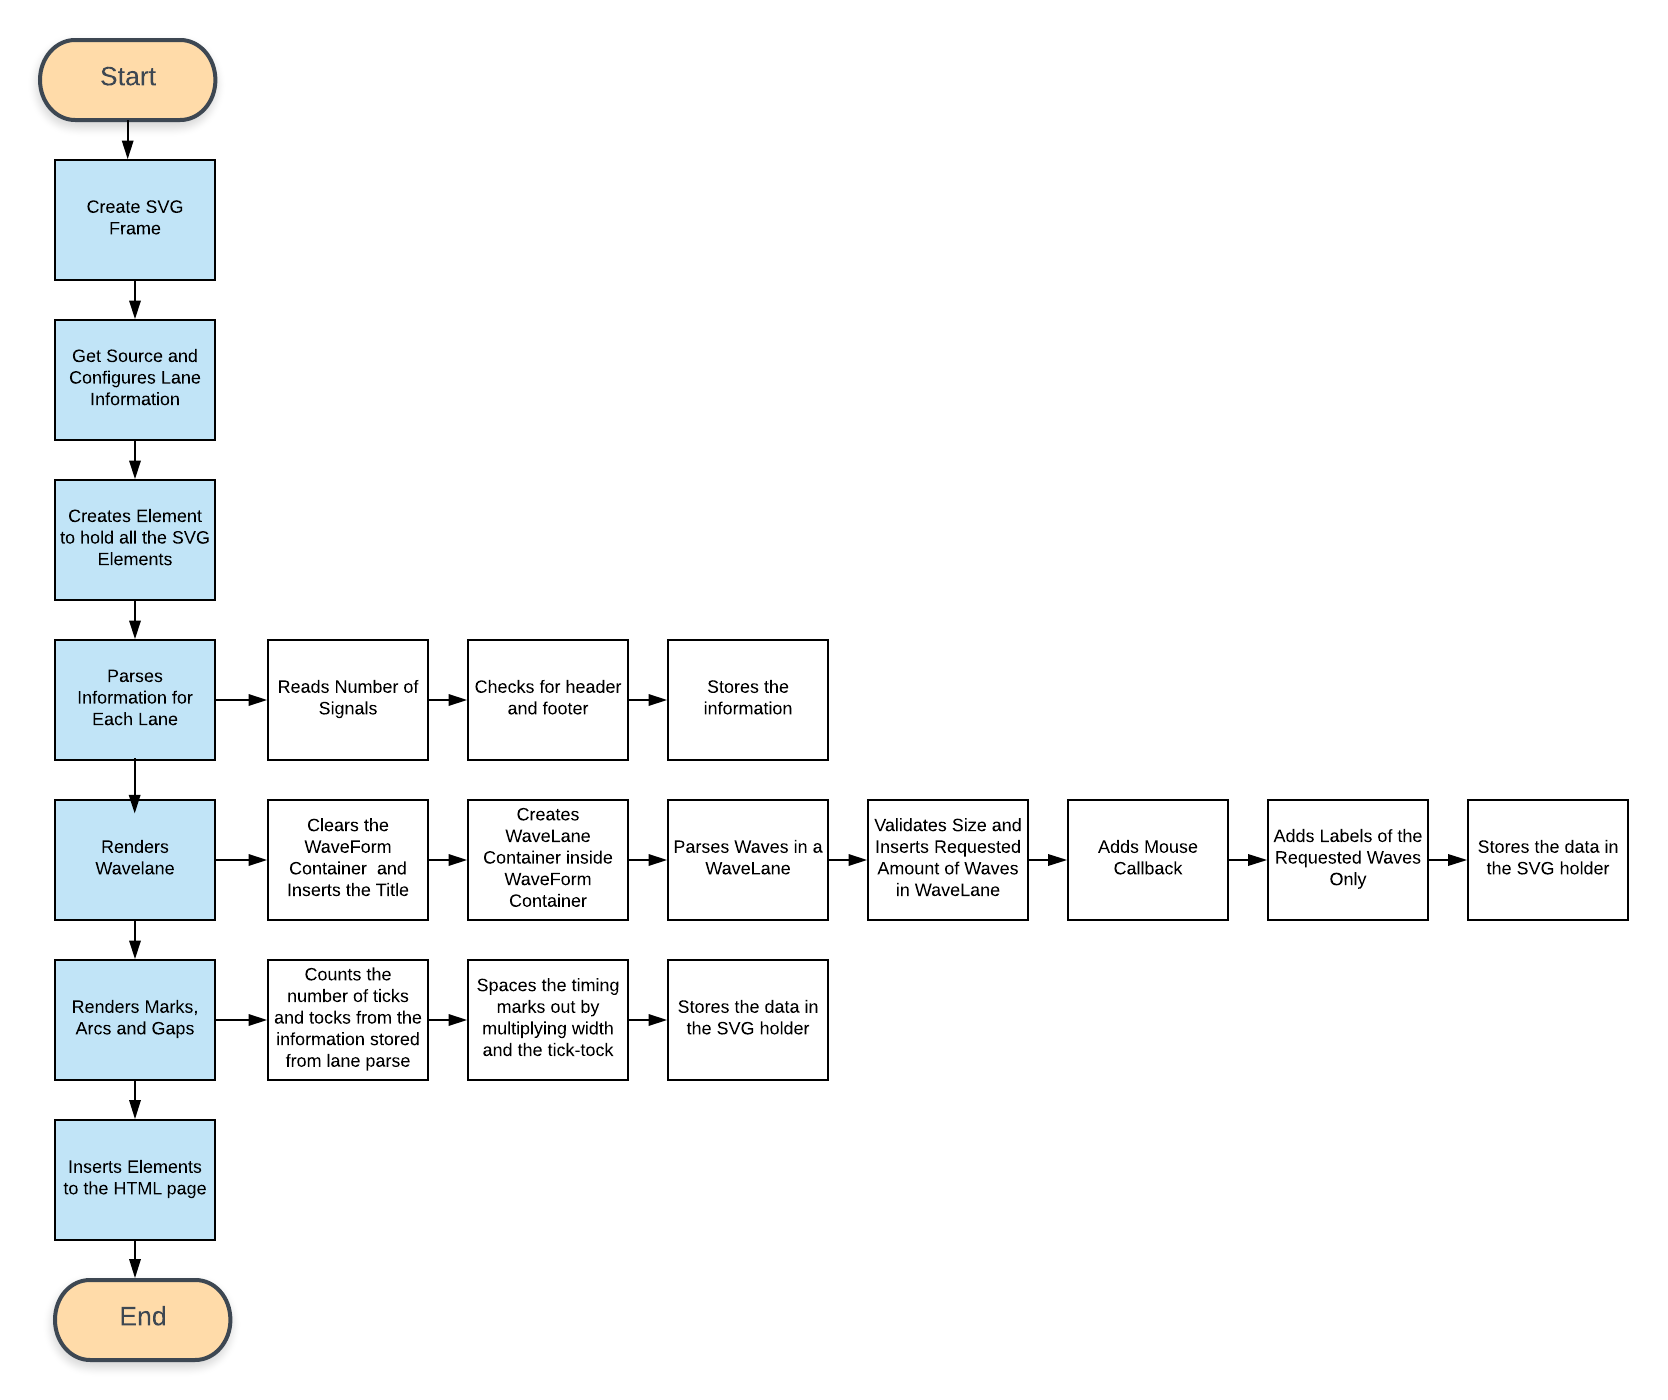
\includegraphics[scale=0.23]{render}
    \caption{Client Side Rendering}
    \label{fig:Client Side Rendering}
\end{figure}
Client side rendering is done using a slightly modified version of the wavedrom library. More about the rendering components has been discussed in Visualization Interface section.
When the server sends the clientdata element that contains the json variable of the selected chunk requested by the client and the client receives it, the data is then processed by the rendering library. To render the waves from text and HTML component called SVG is used. It's a method to draw items on HTML canvas using vectors and often used for graphical interfaces. First an SVG frame is created to hold all of the wavelanes, waves, data, arrows etc. This frame is a holder for all the components and will be inserted into the visualization pane of the HTML file once a page refresh or process method is invoked. After the SVG frame is created, the json data which contains the source and lane information is parsed and separated. 
\par Then an SVG container is created and from the source lane information is parsed individually for each lane. During this process, number of signals or wavelanes are counted and header and footer is looked at. In this phase, necessary calculations are done to fit the render requirements.
\par For the case when a new SVG element is created the SVG container doesn't need to be cleared out for older child elements but when a new data comes in for an ongoing session, the child elements are needed to be removed from the SVG container to put in the elements from the new data. Then two elements are created for the SVG container - title holder and wavelane holder. The title holder holds the name of each of the wavelanes defined in the WaveJSON file. In the case of tight visualization code, the title is autogenerated by the number of elements and they are named as I-0, I-1, etc.
\par In the wavelane holder, elements of the signal object from the json variable will be parsed. The waves are textually defined by their properties in the variable and they are decoded in the render library with pre existing map. A map holds the relation between the text definition of a wave and it's corresponding SVG name. The property of the wave is then parsed from the waveskin files. A waveskin file is a map to the signal name and it's correspnding SVG vectors which would be inserted as an HTML element. It would be described in details for zoom and rendering. 
\par For one wavelane, not all the waves would be rendered on screen as it would take a lot of compute power and would often freeze the web browser to run the render. Based on the user input, the client would only request to render a window of data at a time. When requested, the render library would try to validate the window and render that amount of data only. Rest of the data would be left until further request. At the beginning when the server is requested to send the chunk of data needed by the client, the server sends all the wave information at once to the client. This makes the process run realtime without the need for contacting the server every single time a client requests a horizontal navigation to the left or right. Also since not all the data is being rendered at once, it also cuts down latency significantly.

\par After the wave information is parsed and the vectors associated to the waves are collected, mouse callbacks are added to the waves. This would help the user see the the wave properties as a pop up toast at the bottom of the screen when hovered over the wave, or in the case when an individual wave is clicked it would be selected and highlighted. More details about the mouse callback is mentioned in the section Use. After the mouse callback, if any of the wave has associated labels those are also placed as vectors alongside the waves. This entire process is run for all the wavelanes for the current window. Finally all of the waves are inserted in their associated wavelanes and all the wavelanes are inserted into the SVG container. Anytime the user requests a change, the wave window is refreshed and the SVG items are rerendered. This saves a lot of time and data for the user, since it happens locally.

 
\par Part of the rendering could be saved as an SVG image so that the user can use it for documentation and future references. When the user sends a request to store the file, the entire wave window containing the waves and labels as vectors and exported as a xml file in svg format. Then it is downloaded as a file and when opened, the browser parses this as an xml file and displays it as an image.
 
\par Each of the waves are tied to 2 mouse callback events - click and hover. When a wave is hovered over, it retrieves the ID of the wave and displays it on the screen. For the developers, if they would like to add more properties to the display, they would need to modify the function renderWaveLane to fit their needs.

\par Each wave can also be clicked and highlighted. This option is available to select a reference point for a wave so that when a user is navigating through waves and would like to find out the reference point, it is easily visible from the color. When a selection is requested the render library pushes the id of the wave to a map that holds the id of all the selected waves for the current session and when a change is requested the renderer looks for the selected id from the map on the SVG container. If any of the IDs are found, they are highlighted. If a highlighted wave is selected, then it is removed from the map and the wave is deselected.

\par Zoom is rendered in two different formats - with different skin files (that preserves wave selections) and with horizontal scale (which doesn't preserver selection when zoom level is changed). A skin  file contains a map of WaveJSON data to SVG vector which is loaded into the render to get the sizes of the vectors. For each skin file, these vectors are constant. When the user requests to zoom in or out, different skin files with varity of sizes will be loaded to show different levels of zoom. One downside to this is that, client would have to request all the skin files to depict different zoom levels. Also since the files are quite big, it's hard to edit and create different zoom levels. However, this allows the user to select a wave and zoom in and out without losing the selection.

\par Another way to zoom is using hscale, which is the preferred method. In this method when the user requests to zoom in or out, the clients looks at the initially loaded skin file and then it requests the reneder to expand all the waves, marks and arc on the horizontal axis and to render for a smaller window size. This way only one skin file would be used and it would cost much less data for the user.




\newpage
\section{Visualization Interface}
\subsection{Text Format}
A typical WaveJSON text contains the parent variable signal. The signal variable is an array that contains wave, edge, groups, arrows, config, head \& foot. A wave is a variable which usually has the attributes name and data along with the wave signal. name is the title of the wavelane or a set of waveforms in a horizontal line. data is an array of string that attributes the data in multibit waves like this

\begin{figure}[H]
    \centering
    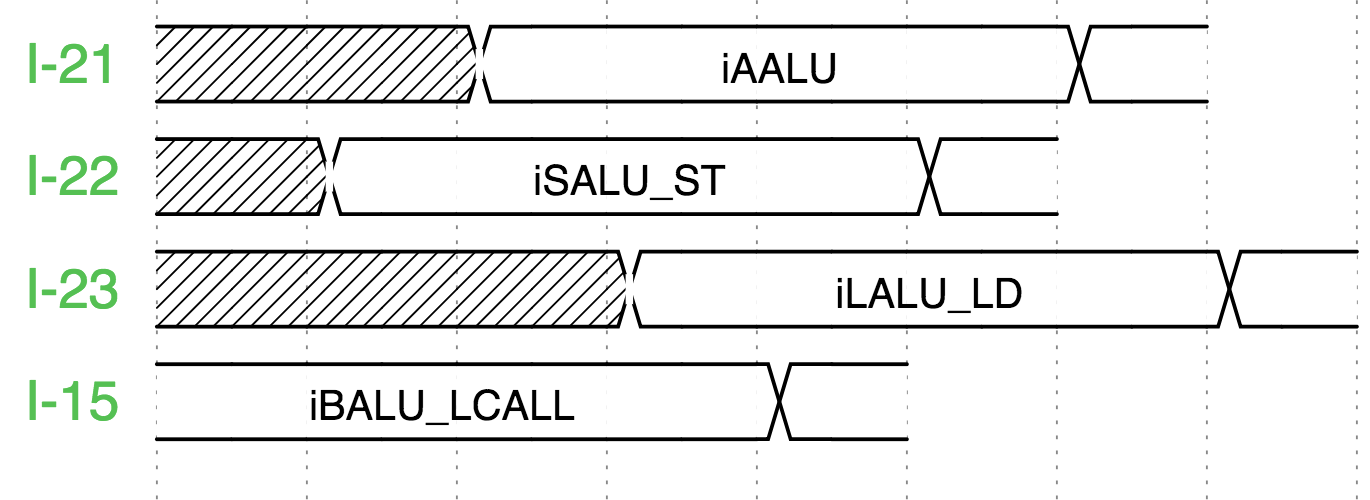
\includegraphics[scale=0.7]{wave}
    \caption{Multibit Wave with Data}
    \label{fig:wave_data}
\end{figure}

edge  contains an array of spline and straight arrow connotations which are often useful to mark important clock edges. Pclk, Nclk are used to connotate rising edge and falling edge like this

\begin{figure}[H]
    \centering
    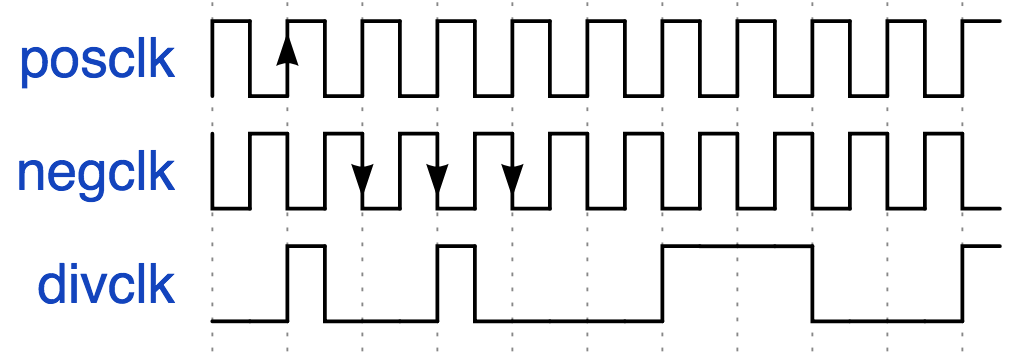
\includegraphics[scale=0.7]{clock}
    \caption{Clock Edge}
    \label{fig:clock_edge}
\end{figure}

groups are ways to cluster number of wavelanes together. For example, master and slave waveforms can be displayed in the same window by tagging the wavelanes as following which would potentially help distinguish and differentiate between the two types of waveforms.

\begin{figure}[H]
    \centering
    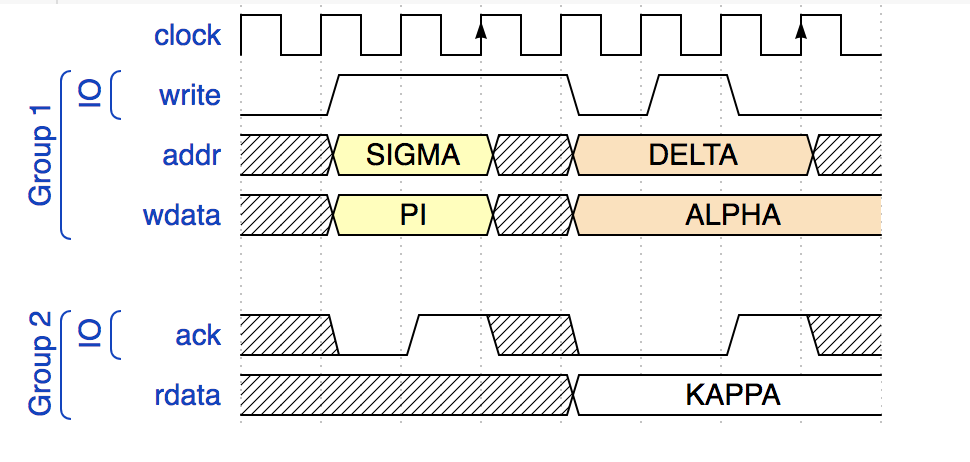
\includegraphics[scale=0.7]{groups}
    \caption{Groups}
    \label{fig:groups}
\end{figure}

arrows are ways to mark between wavelanes and wave cycles. Using arrows we can tag necessary execution time between two cycles, dependencies or faults in the waveforms like 

\begin{figure}[H]
    \centering
    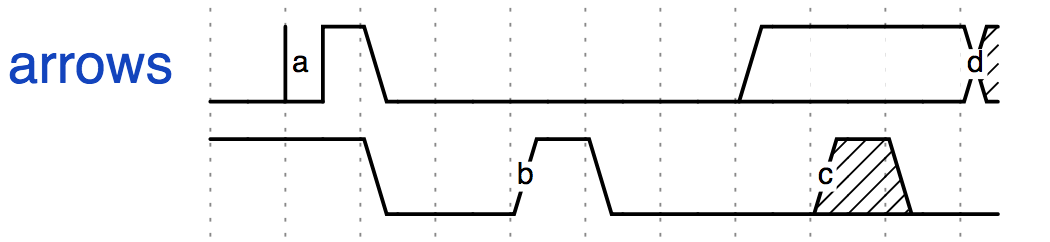
\includegraphics[scale=0.7]{arrow}
    \caption{Arrows}
    \label{fig:arrow}
\end{figure}

gaps are ways to skip recurring and similar waveforms which doesn't change throughout multiple waves in a wave diagram. Instead of printing all of them individualy, gaps connotation can be used in all of them to skip a certain time period where the given waves showed a constant behavior. It is useful to visualize the data without the need to navigating the wave left or right.

\begin{figure}[H]
    \centering
    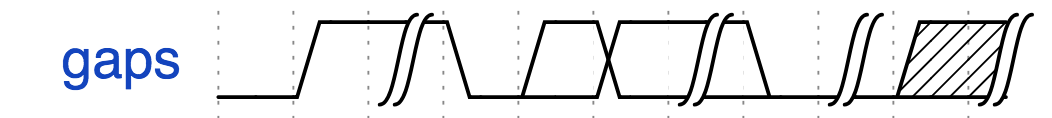
\includegraphics[scale=0.7]{gaps}
    \caption{Gaps}
    \label{fig:gaps}
\end{figure}

config, head and foot are part of the WaveJSON file which defines the size of the waveforms, lane markers, size of texts, adding header and footer etc.

\subsection{Client Server Interaction}
The backend server is created using nodejs and number of npm packages including http for creating an http webserver, formidable for form handling, fs to access the server file system and parse for parsing files. All of the server side code is written in the express\_server.js file.

 First of all, we would need a way to communicate between the front end website’s user interaction with the back end module by transferring data and vice versa. For that purpose, we defined a variable called clientdata which holds the socketid for the current socket, filename which holds the uploaded wavejson file information, start\_time which defines the beginning of the timing diagrams current position and window\_size which defines how many wave blocks can fit in the window, v\_start\_time which defines the beginning index of the wavelanes displayed in the current window and v\_size which defines how many wavelanes will be shown in the current window, source\_size that defines how many wavelanes are in the source file, and code\_text is used to post the code written in the text box for tight visualization.
 \par Then we set up a mechanism for data handling. We set up an http server and tie a file handler to it so that we can receive the file posted by the user. For that we can use the npm express and file-upload modules over HTTP POST request. We also use the socket.io npm module to keep the live communication between the client and the server without using HTTP GET or POST requests so that a page refresh or redirection is not needed to handle any user interaction.
 \par When a client tries to connect to the server and the server module is running, the express server will send the index.html, default.js, index.css files to the client which is parsed by the client browser as the web interface (details about these files are written in the Front End Architecture section). Waveform visualization could be done in 2 ways - displaying a waveJSON file and displaying tight visualization. When a post request is made by the client, the server checks the requests to see if a file has been uploaded. If there is no file, then it checks for the text for tight visualization. If neither are found then the server would return an error code. If a file is found then it is moved to the tmp directory and renamed according to the current socket name. If visualization text was uploaded then  the text is splitted by new lines and evaluated accordingly. After the file or the text upload is complete, the user is redirected to index.html with parsed file data. In both cases the text is evaluated by JavaScript and converted into a JSON variable. Then it’s passed to the client with redirection. If for any reason there is an error in the evaluation, the server will return an empty variable and web interface would not show any visualization.
 \par Next, we have client interaction handling. There are 4 different interactions which can be performed by the user that can modify the visualization by updating the JSON variable. These 4 interactions are shifting the time diagram to the left, shifting to right, changing the wavelanes shown in the window by moving up and down. When the client presses the respective button for any of these actions the variables v\_start\_time, v\_size, start\_time, and window\_size are updated accordingly which is sent to the server. The server then parses the json file or the tight text based on the value of the above variables and sends the resultant json string back to the client. For example, v\_start\_time= 6, v\_size=10, start\_time=29, and window\_size = 20 the server will parse the json file to see if there are at least 16 wavelanes/signals. If there are 16 or more signals then the server will send signal 6 to 15 back to client and the waveform will start from the time 29 and end at 48.

\subsection{Parsing}
 The front end or the client side system is based on WaveDrom and is modified to fit the socketio integration. There are two parts of the system. The first one is the client html file with the socket implementation and the second part is the wavedrom library. At first the client initiates a socket connection with the server which is called by the function bodyload. 
 \par If the client had never accessed the website, then it will initiate a new connection and store that information in the browser cache. If the client had previously uploaded a file or tight code in the text box then it will be fetched from the browser cache and loaded in the browser. When the client uploads a WaveJSON file with the signal , it’s evaluated by the server and the requested chunk of the waveform is sent back to the client as a JSON variable. Then the function processAll is called which calls the function renderWaveForm and passes the JSON variable to it. The signal is then validated and the wavelanes are parsed. After that the function renderWaveLane is called to turn the source signal text into SVG contents for display. From there, gmarks are rendered in the  wavelanes followed by vertical timing marks, arcs, and texts are rendered.

\section{User Manual}
\subsection{Installation}
 	MASCWave server is npm based so to install it, Node JS needs to be installed to the server and the following packages needs to be installed by running 
 
 \begin{minted}{bash}
 	npm install --save [PACKAGE_NAME]
\end{minted}	
    \textendash body-parser,\\
    \textendash http,\\
    \textendash csv-string,\\
    \textendash express,\\
    \textendash express-fileupload,\\
    \textendash fs,\\
    \textendash path,\\
    \textendash socket.io,\\
 After that cloning from this git repository \url{https://github.com/kabylkas/mascwave} should get it in the server.
 
 \par Alternatively if the npm module npm-install-all could be used to install all the dependecies listed in package.json file. To install and npm-install-all, the user would need to run the following commands.
 
 \begin{minted}{bash}
            npm install -g npm-install-all
            cd [SERVER_DIRECTORY]
            npm-install-all
\end{minted}

    
\subsection{Use}
\begin{figure}[H]
    \centering
    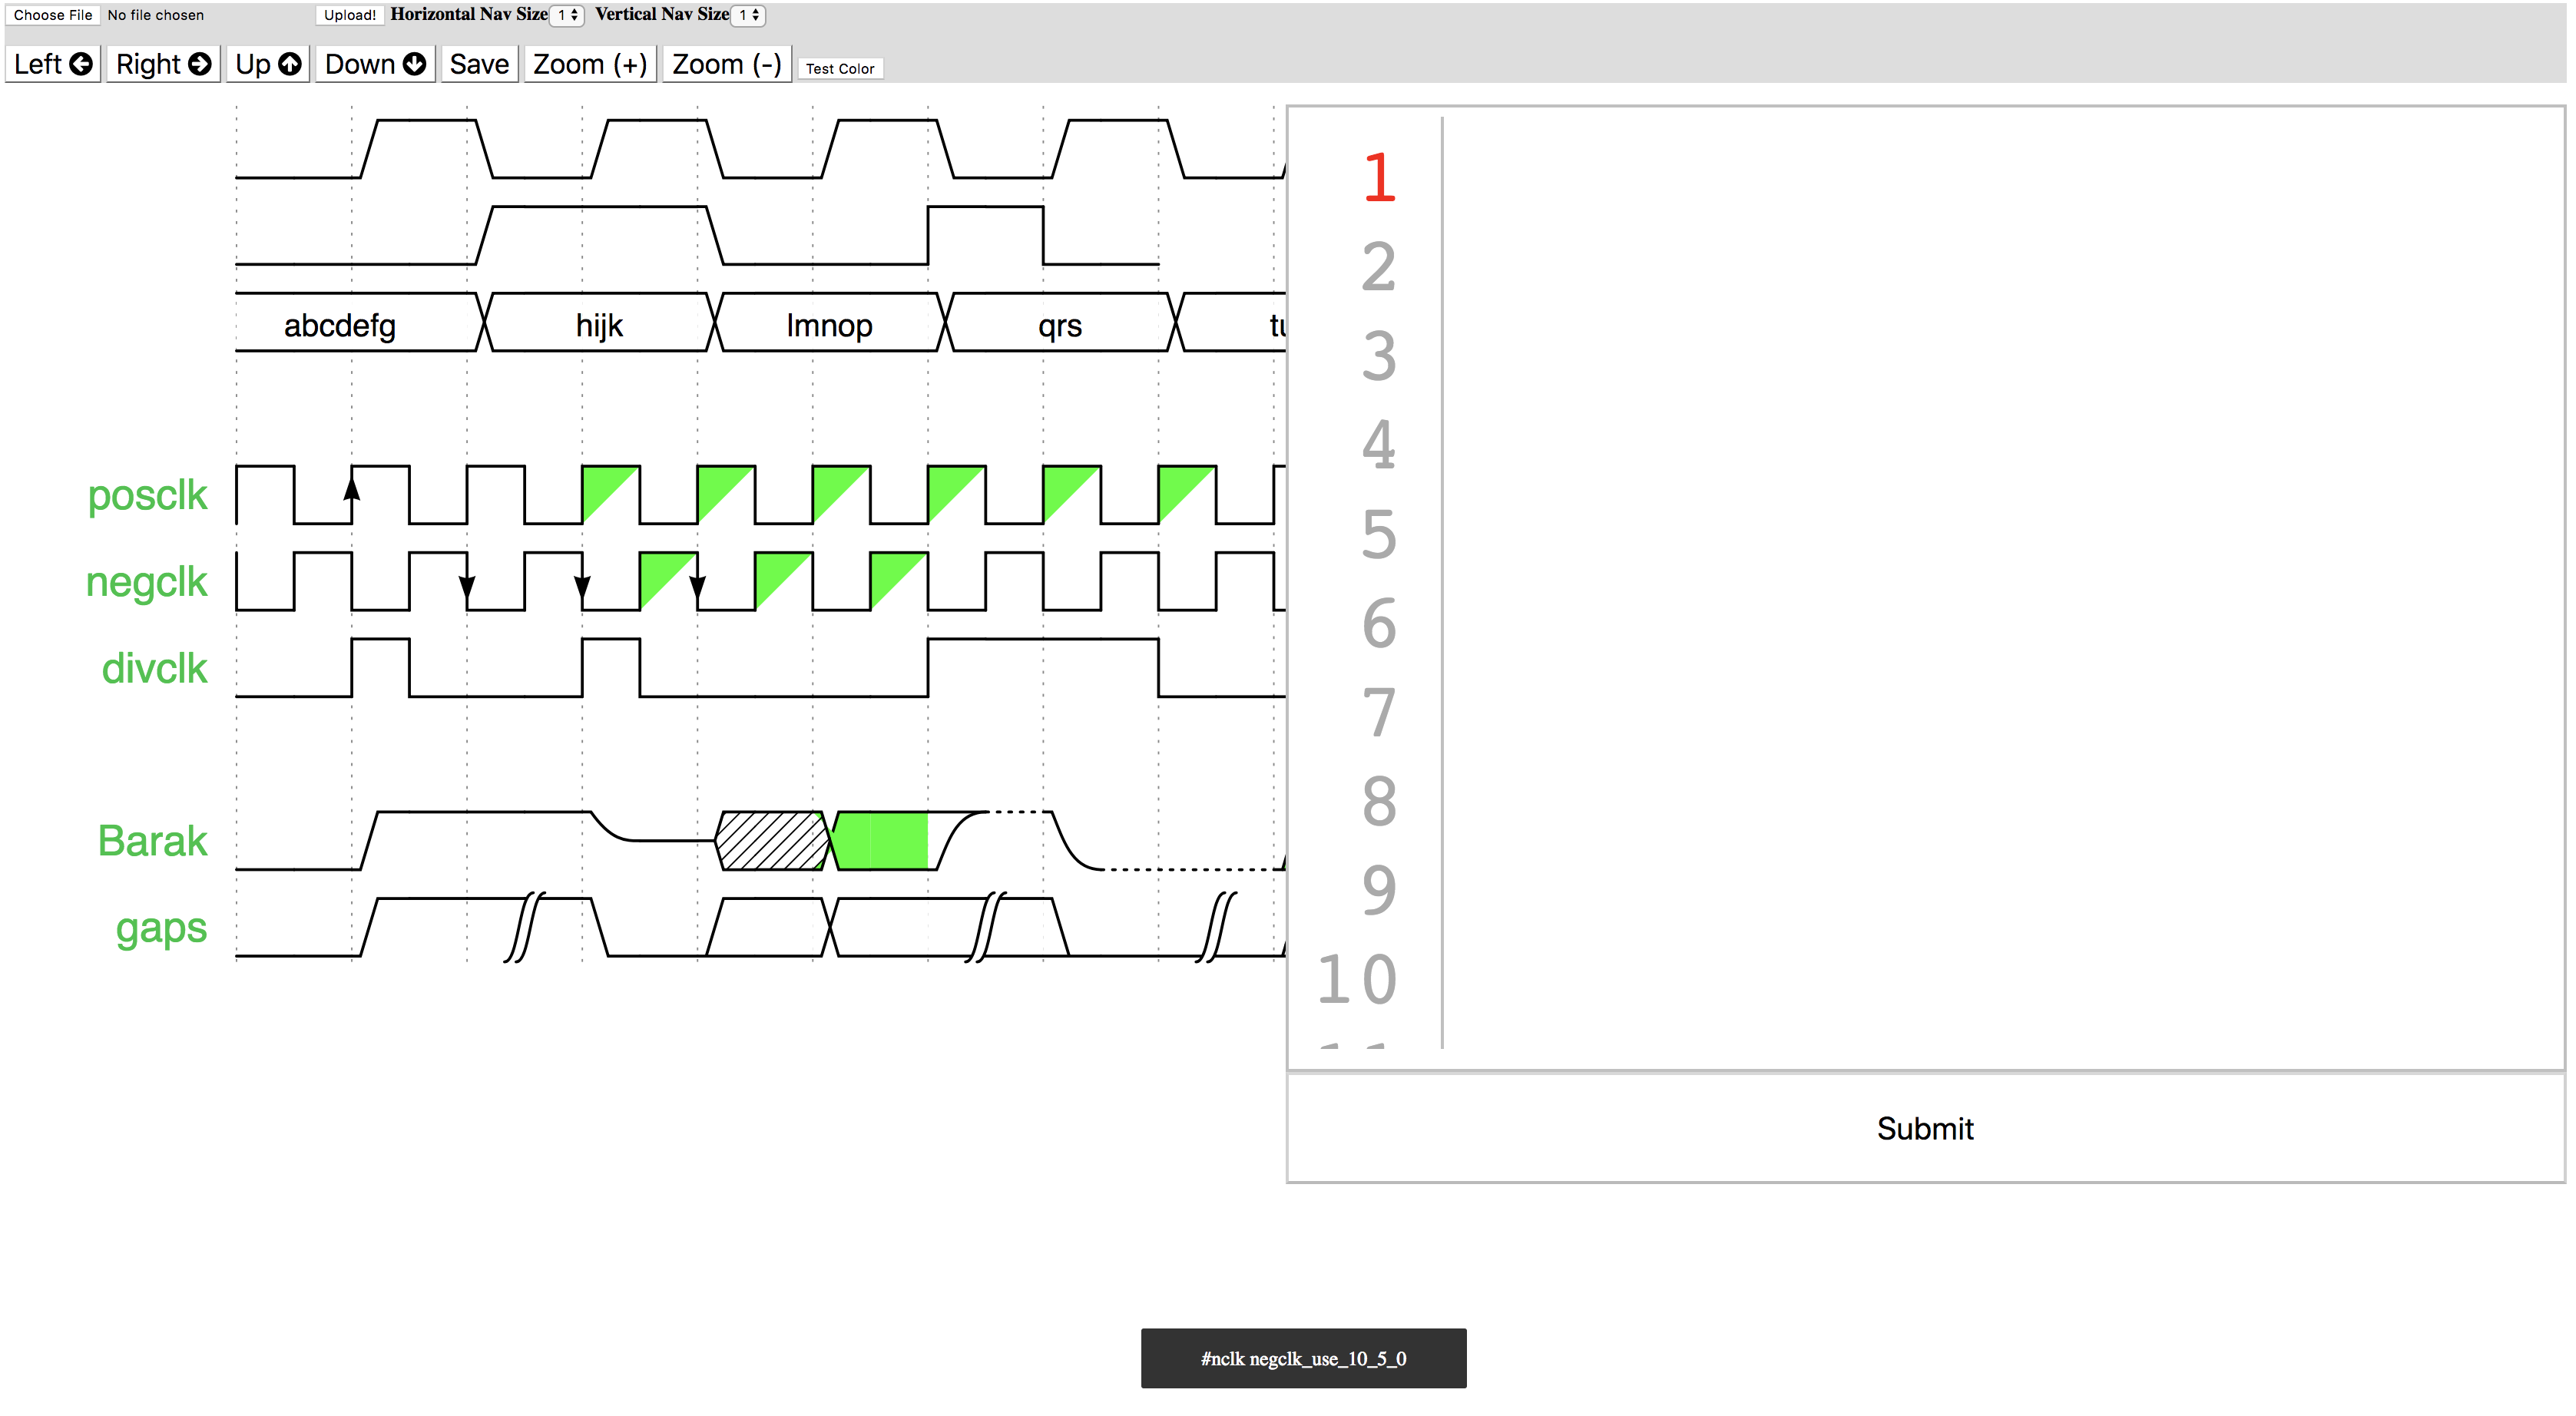
\includegraphics[scale=0.3]{tutorial}
    \caption{Screen Shot of a Sample WaveForm}
    \label{fig:tutorial}
\end{figure}
 MASCWave is simple to use. Once the server is setup, the client would need to get the server URL. On the server side user needs to run npm start from the project directory.
\subsubsection{Upload a file}
 The user can click on Choose File and select a WaveJSON file, then click Upload. As long as the file content is properly formatted as WaveJSON, the waveform will be generated in the left pane.
\subsubsection{Submit Code}
 The user can write javascript code and that would be evaluated by the server and waveform will be generated so long the function or chunk of code returns an array. Otherwise it would return undefined.
\subsubsection{Navigate Horizontally}
 To Navigate to the right to view more of the waveform, user can click the right button on the top or simply use their right arrow key on the keyboard as long as the code pane on the right isn’t selected or doesn’t have a cursor on it. To navigate to the left, the user can use the left button or the left arrow key.
\subsubsection{Navigate Vertically}
 If there are multiple wavelanes that didn’t fit in the current window, the user can navigate to top or bottom using the button on screen or using the up/down arrow keys on their keyboard.
\subsubsection{Selecting and Deselecting Waves}
 To select a wave the user can click on the wave which will highlight it with green color and clicking again will deselect it.
\subsubsection{Saving File}
 By Clicking the button Save, users can download and save the current view of the waveform.
\subsubsection{View Wave ID}
 The ID of the wave will be visible when the user hover their mouse over it. A toast will pop up at the bottom of the screen.
 \subsubsection{Zoom In and Out}
 To resize the wave forms, users can use the Zoom in and Zoom out button to give them more visualization of the data without the need of navigation on the horizontal lane. Currently there are 2 zoom levels implemented. In the future, more waveskins could be introduced allowing more levels of zoom to be accepted.
 \subsubsection{Navigation Size Select}
 The navigation size could be controlled by the input given by the user. For example, if the users want to shift the waveform by 1 clock cycle every time they input a horizontal shift command, they can select the horizontal navigation size to 1 and it is updated to fit the input. So every time the user gives a horizontal navigation input the wave will shift by one clock cycle to the given direction. Similarly, setting the vertical navigation size will determine the navigation amount to view more wavelanes.
 \newpage
 \section{Future Work}
 \par As of now, when the server sends back chunk of data to the client, it only chops the data on the vertical view, which means if there are 100 waves the server will chop the wavelanes in groups and send only 10 lanes at a time. It doesn't chop the horizontal data on each of the selected lanes since that doesn't take more than a couple bytes usually. Typically the render would only render the amount of horizontal data based on the window location and would disregard the rest thus it doesn't take more computation power and runs it in real time. However, it isn't optimizing the amount of data being sent to the client if each of the wavelanes have significant amount of data then eventually it would cost the client for network even the data is compressed. So in the future, we need to implement a way to crop and send data per wavelane as well.
 \par As of now there are only 2 zoom modes namely zoom in and zoom out. Since the zoom mode for SVG contents would depend on the waveskins, if we could have more waveskins of different sizes then we can have many different sizes of zoom capability. Currently, the only two waveskins are narrow and default.
 \par Currently, there is no log in method implemented for the system but in the future, we can have a log in system for clients so that each individual can store multiple wave files to their accounts and save network data by not reuploading the same file over and over. Also they would also be able to share their files to their peers saving them network data as well.
 \par As of now, the system has bare minimum security associated to it, since hacking into a websocket isn't as easy as a man in the middle, ping or injection attack. But in the future there should be encryption associated because it might be hard to break into a websocket but it isn't impossible.
 
\newpage
\section{Conclusion}
 MASCWave is an great online tool for visualization of waveform. It is HTML5 based so no extra plugin is necessary and could also be viewed from mobile devices. This works with most major browsers like Chrome, Safari, Firefox and Explorer 11. Currently it is well supported for WaveJSON files only but in future we will try to fit in as many formats as possible. Also future work plan includes modification of waveskin to show selected waves neatly, compressing the data communicated between client and server, extend support to all web browsers, and make server side installation process easier.
\end{document}

